%%%%%%%%%%%%%%%%%%%%%%%%%%%%%%%%%%%%%%%%%
% University/School Laboratory Report
% LaTeX Template
% Version 3.1 (25/3/14)
%
% This template has been downloaded from:
% http://www.LaTeXTemplates.com
%
% Original author:
% Linux and Unix Users Group at Virginia Tech Wiki 
% (https://vtluug.org/wiki/Example_LaTeX_chem_lab_report)
%
% License:
% CC BY-NC-SA 3.0 (http://creativecommons.org/licenses/by-nc-sa/3.0/)
%
%%%%%%%%%%%%%%%%%%%%%%%%%%%%%%%%%%%%%%%%%

%----------------------------------------------------------------------------------------
%	PACKAGES AND DOCUMENT CONFIGURATIONS
%----------------------------------------------------------------------------------------

\documentclass{article}

\usepackage[version=3]{mhchem} % Package for chemical equation typesetting
\usepackage{siunitx} % Provides the \SI{}{} and \si{} command for typesetting SI units
\usepackage{graphicx} % Required for the inclusion of images
\usepackage{natbib} % Required to change bibliography style to APA
\usepackage{amsmath} % Required for some math elements 
\usepackage{glossaries} % For acronyms
\usepackage[bookmarks]{hyperref} %Bookmarks for pdf
\setlength\parindent{0pt} % Removes all indentation from paragraphs

\renewcommand{\labelenumi}{\alph{enumi}.} % Make numbering in the enumerate environment by letter rather than number (e.g. section 6)

\usepackage{times} % Uncomment to use the Times New Roman font

\usepackage{listings} % Required for inserting code snippets
\usepackage[usenames,dvipsnames]{color} % Required for specifying custom colors and referring to colors by name

\definecolor{DarkGreen}{rgb}{0.0,0.4,0.0} % Comment color
\definecolor{highlight}{RGB}{255,251,204} % Code highlight color

\lstdefinestyle{Style1}{ % Define a style for your code snippet, multiple definitions can be made if, for example, you wish to insert multiple code snippets using different programming languages into one document
language=XML, % Detects keywords, comments, strings, functions, etc for the language specified
backgroundcolor=\color{highlight}, % Set the background color for the snippet - useful for highlighting
basicstyle=\footnotesize\ttfamily, % The default font size and style of the code
breakatwhitespace=false, % If true, only allows line breaks at white space
breaklines=true, % Automatic line breaking (prevents code from protruding outside the box)
captionpos=b, % Sets the caption position: b for bottom; t for top
commentstyle=\usefont{T1}{pcr}{m}{sl}\color{DarkGreen}, % Style of comments within the code - dark green courier font
deletekeywords={}, % If you want to delete any keywords from the current language separate them by commas
%escapeinside={\%}, % This allows you to escape to LaTeX using the character in the bracket
firstnumber=1, % Line numbers begin at line 1
frame=single, % Frame around the code box, value can be: none, leftline, topline, bottomline, lines, single, shadowbox
frameround=tttt, % Rounds the corners of the frame for the top left, top right, bottom left and bottom right positions
keywordstyle=\color{Blue}\bf, % Functions are bold and blue
morekeywords={}, % Add any functions no included by default here separated by commas
numbers=left, % Location of line numbers, can take the values of: none, left, right
numbersep=10pt, % Distance of line numbers from the code box
numberstyle=\tiny\color{Gray}, % Style used for line numbers
rulecolor=\color{black}, % Frame border color
showstringspaces=false, % Don't put marks in string spaces
showtabs=false, % Display tabs in the code as lines
stepnumber=5, % The step distance between line numbers, i.e. how often will lines be numbered
stringstyle=\color{Purple}, % Strings are purple
tabsize=2, % Number of spaces per tab in the code
}

\newcommand{\insertcode}[3]{\begin{itemize}\item[]\lstinputlisting[caption=#2,label=#3,style=Style1]{#1}\end{itemize}} % The first

\newacronym{ssm}{SSM}{Survey State Model}
\newacronym{xml}{XML}{Extensible Markup Language}

%----------------------------------------------------------------------------------------
%	DOCUMENT INFORMATION
%----------------------------------------------------------------------------------------

\title{Survey State Model (SSM)\\ Authoring language of electronic questionnaires} % Title

\author{Jose Lloret - jose@pexel.co.uk} % Author name

\date{\today} % Date for the report

\begin{document}

\maketitle

% If you wish to include an abstract, uncomment the lines below
% \begin{abstract}
% Abstract text
% \end{abstract}

\section{Introduction}
Survey research is the systematic collection of information from individuals and organisations to address research and/or business objectives. This social science is formed by five stages (see Figure \ref{fig:5stage}) and allows the identification of market demands, detection of opportunities or customer preferences understanding among others.
\begin{figure}[h!]
\label{fig:5stage}
\centering
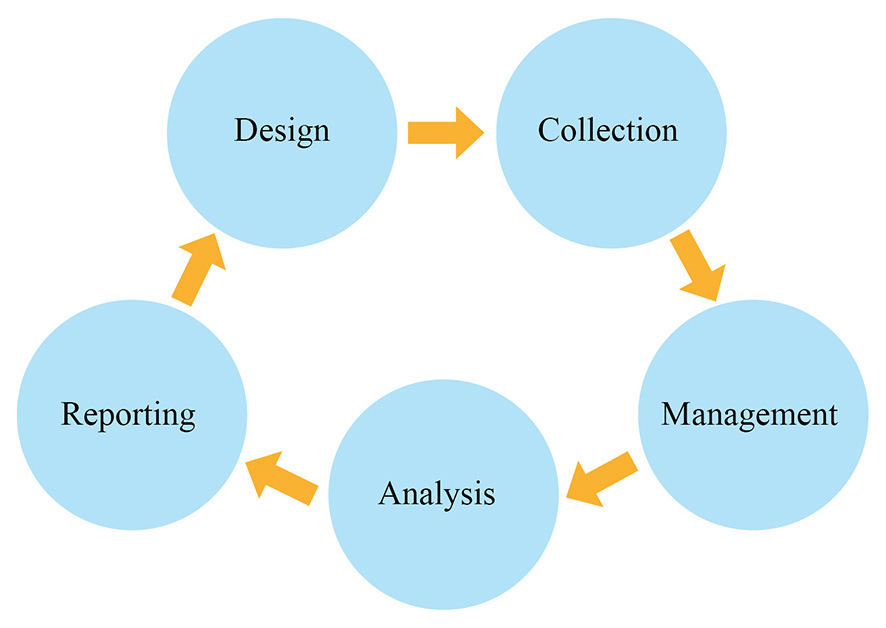
\includegraphics[width=0.75\textwidth]{img/5stage}
\caption{5 stages process for surveys}
\end{figure}
This manual is intended to describe the most frequent features from surveys through \gls{ssm}. This language follows a state-transition approach to describe the flow of questionnaires and improves the existing \gls{xml} languages to describe questionnaire's constructs by adding personalisation features.
\section{Survey metadata}
Survey metadata section of \gls{ssm} permits describing the name, description and date for a survey. Listings \ref{lst:metadata} defines an example of metadata according to \gls{ssm}.
\insertcode{"scripts/metadata.xml"}{Metadata for surveys}{lst:metadata}
\section{Survey content}
Survey content is structured with sections. A section allow grouping questions and permits reusing it several times when it is referenced in a composite state (see Listing \ref{lst:section}). There are five types of questions that can described in \gls{ssm}: intro, single, multiple, open and grid, following subsections will explain them in detail.
\insertcode{"scripts/section.xml"}{Sections structure}{lst:section} 
	\subsection{Intro question}
	Intro question not only becomes useful to introduce the respondent to a new section but also can be used for ending a survey with a customised message. Listing \ref{lst:intro} defines an intro question whose name is INF and there is a label defined in English to describe the content that would appear during the collection stage. 
\insertcode{"scripts/intro.xml"}{Intro question example}{lst:intro}
	\subsection{Single question}
	Single question asks the respondent anything in which one and only one response from the set can be chosen. Listing \ref{lst:single} represents a single question whose name is Q0, contains one label in English and four possible responses, one closed and three open. 
\insertcode{"scripts/single.xml"}{Single question example}{lst:single}
A single question could be "What is your favourite colour?, "How many times do you read newspapers per week?" or "What percentage do you expect to increase on sales this year? where verbatim responses from the respondent could help to get accurate results and respondent's opinion, as such \gls{ssm} offers the open response types string, integer or decimal (e.g. codes 2, 3 and 4 respectively) to satisfy this level of personalisation.
	\subsection{Multiple question}
	Multiple question permits the respondent to choose one or more responses from the set. Listing \ref{lst:multiple} asks expectations from work and there is a minimum and maximum limit to choose (e.g. 1 and 3 respectively) from the set of 5 responses. Also, each response can be exclusive meaning that is not affected by the limit.
\insertcode{"scripts/multiple.xml"}{Multiple question example}{lst:multiple}
Exclusive response feature becomes useful for responses such as don't know, refuse to ask or prefer not reveal. Similarly to the single question, open response types can be defined in multiple question type too.
	\subsection{Open question}
	Open question allows the respondent answering the question freely. There are three types defined in \gls{ssm} to address survey requirements. One is string or verbatim question addressed to obtain respondent views and becoming extremely useful for sentiment analysis techniques of computing. Listing \ref{lst:open_string} asks for feedback regarding a training session where respondent's opinion may lead to improve things.
\insertcode{"scripts/open_string.xml"}{Verbatim question example}{lst:open_string}
Other type is numeric integer, useful for survey designers if they do not know the possible closed responses. Listing \ref{lst:open_integer} asks the number of people living in a property. Not only min and max limits could be imposed to avoid unexpected responses but also default value response can help when collecting data survey stage takes place.
\insertcode{"scripts/open_integer.xml"}{Numeric integer question example}{lst:open_integer}
Finally, numeric decimal, rarely used, can help to get accurate numbers. Listing \ref{lst:open_decimal} represents a decimal open question.
\insertcode{"scripts/open_decimal.xml"}{Numeric decimal question example}{lst:open_decimal}
	\subsection{Grid question}
	Grid question allows asking more than one thing in the same question. There are three types of grid supported in \gls{ssm} permitting the respondent to choose a single option in each row, allowing them to tick multiple for each row or text boxes for entering numeric responses.

Grid single (Listing \ref{lst:grid_single}) asks three statements where only one response per row is permitted (Strongly disagree, disagree, neither, agree and strongly agree).
\insertcode{"scripts/grid_single.xml"}{Grid single question example}{lst:grid_single}
Multiple grid (Listing \ref{lst:grid_multiple}) asks for each type of soft drink what features the respondent feels where there are no restrictions to pick up (Fun, Sexy and Masculine) for each soft drink.
\insertcode{"scripts/grid_multiple.xml"}{Grid multiple question example}{lst:grid_multiple}
Numeric grid (Listing \ref{lst:grid_numeric}) asks rating the performance for three statements in each company X, Y, Z provided. As the reader may note, it is needed to fill every row and column with a number from 1 to 5. This type of question should be shown to the respondent as a text box for each row/column.
\insertcode{"scripts/grid_numeric.xml"}{Grid numeric question example}{lst:grid_numeric}

\emph{Note that each row of a grid question can be defined as closed or open (string, integer or decimal) whereas the columns are only closed.} Although this could constitute a limit for the language thanks to the transposed feature present in grid questions (rows seen as columns and columns seen as rows) allows the respondent to see open responses as they were in the columns but really they would not be.
\section{Field}
Field section defines the variables that are shared across sections. Fiels are widely used for loop and computation states in the routing section of \gls{ssm}. Listings \ref{lst:field} describes the four types of variables available in \gls{ssm}.
\insertcode{"scripts/field.xml"}{Field examples}{lst:field}
Every variable defined requires an id and value. The value must be according to the type declared, as such the example values are 0.0, 0, "Hello World! matching with the types decimal, integer and string respectively. \emph{Note that iterator variable does not have a value defined since its value is modified through for states of \gls{ssm} routing.}
\section{Survey routing}
In order to describe routing for surveys it is used a state-transition approach. As such, the routing part is composed by statemodels which must refer to sections defined in the content part of \gls{ssm} and an entrypoint marking the starting point of execution, see Listings \ref{lst:routing}. Every statemodel contains states that can be \emph{simple}, \emph{composite} or \emph{pseudo}.
\insertcode{"scripts/routing.xml"}{Routing example}{lst:routing}
 Below, there are explained the different states available to describe routing features:
	\subsection{Simple}
	Simple states are those addressed to interact with the respondent because they are able to retrieve questions that are defined in the content part. For instance, Listings \ref{lst:simple}
\insertcode{"scripts/simple.xml"}{Simple state example}{lst:simple} 
contains a simple state (s0) which contains one variable whose reference is a single question defined in the section 1 of the content. When this state is left, that is the respondent press forward or next, the state reached should be p0.
	\subsection{Composite}
	Composite states are able to reuse other statemodel. Listings \ref{lst:composite} defines the state c0 as composite which embeds the statemodel 1 in the statemodel 0, that is the statemodel 0 executes the behaviour from the statemodel 1 when c0 is reached.
\insertcode{"scripts/composite.xml"}{Composite state example}{lst:composite}
Composite states become useful when they are combined with For states (see Section \ref{subsec:for}).
	\subsection{If}
	If states are used to describe flow through the survey, in other words, what path to take whether the expression is satisfied or not. Listings \ref{lst:if} describes a filter to decide whether going to sink0 state or s2. The logical expression (written in postfix mode) would be true if the respondent selected "no" from Q0. Bear in mind that not only every variable referenced in the expression must be defined in the section pointed by the statemodel but also the target transitions have to be states specified in the statemodel, otherwise the \gls{xml} file is not valid according to \gls{ssm}.
\insertcode{"scripts/if.xml"}{If state example}{lst:if}
	\subsection{Check}
	Check states are addressed to validate any inconsistence stopping the flow if the logical expression is not valid. Check state can be either \emph{warning} or \emph{error} giving the possibility to continue responding the survey or stopping until the inconsistence is solved respectively. Listings \ref{lst:check} defines an error check which validates whether never was selected in Q3a or not.
\insertcode{"scripts/check.xml"}{Check state example}{lst:check}
The above check only validates that never is selected in Q3a but it is needed a previous if state to decide whether reaching the check or not according to the respondent age, otherwise the check state would become false for any response different to never in Q3 without taking into account respondent's age.
	\subsection{For}
	For state is used to indicate that a statemodel has to be repeated a number of times, in other words, to repeat the questions of a section as many times as the expression is satisfied. There are three types of iterations: \emph{range}, \emph{expression\_list} or \emph{list}. The range iterator accepts integer operands coming from constants, variables or expressions returning an integer operand. Listings \ref{lst:forRange} describes a for state whose iterator is range.
\insertcode{"scripts/for_range.xml"}{Range for state example}{lst:forRange}
In order to describe a range iterator it is needed:
\begin{itemize}
	\item \emph{field} referring to an iterator variable defined in the field section. This variable can be used for text piping for questions since the same question can be repeated many times so knowing in what position is the iterator permits its unique identification.
	\item \emph{range start} marks the beginning of the iterator. Usually the start element is a constant integer 0.
	\item \emph{range end} sets the ending of the iterator. The example provided refers to an open integer question.
	\item \emph{range step} indicates the increments to perform in each iteration. Usually is a constant integer 1.
	\item \emph{true transition} requires a composite state without transition to avoid cycle loops. The for state will create a new 
statemodel for each iteration of the loop.
	\item \emph{false transition} is the successor state when the iteration loop ends.
\end{itemize}
The expression\_list iterator accepts expressions which return a list such as selected/unselected/all choices from single/multiple question(s). Listings \ref{lst:forExprList} describes a for state whose iterator is an expr\_list.
\insertcode{"scripts/for_expr_list.xml"}{Expression\_list for state example}{lst:forExprList}
In order to describe a expr\_list iterator it is needed:
\begin{itemize}
	\item \emph{field} referring to an iterator variable defined in the field section. This variable can be used for text piping for questions since the same question can be repeated many times so knowing in what position is the iterator permits its unique identification.
	\item \emph{expr\_list} permits defining any kind of expression which returns a list. The example provided is retrieving the responses selected in Q7 to create the iterator but other combinations such as unselected in Q7, all choices in Q7, selected in Qx union unselected in Qy and so on are possible. \emph{Note, every variable referred in the expression list must be a defined single or multiple question in the section pointed by the statemodel.}
	\item \emph{true transition} requires a composite state without transition to avoid cycle loops. The for state will create a new 
statemodel for each iteration of the loop.
	\item \emph{false transition} is the successor state when the iteration ends.
\end{itemize}
Finally the list iterator refers to a list variable defined in the field section. \emph{Note that this type of iterator is still not implemented in the collection stage of surveys.}
	\label{subsec:for}
	\subsection{Computation}
	Computation state can be used to specify intermediate operations that are carried out during the execution of the survey. Basically, this state performs an arithmetical operation over a variable defined in the Field section. Listings \ref{lst:computation} adds one to the working variable.
\insertcode{"scripts/computation.xml"}{Computation state example}{lst:computation}
\emph{Note, the variable to refer only can be a variable from the Field section. In this case, working is an integer variable.}
	\subsection{Sink}
	Sink states are aimed to describe the ending of a statemodel, that is the ending of a section. For instance, Listings \ref{lst:sink} contains an if state which switches to sink0 if the expression becomes true meaning that sink0 would be the last state to execute in the statemodel 1.
\insertcode{"scripts/sink.xml"}{Sink state example}{lst:sink}
	\subsection{Terminate}
	Terminate states are used to describe the ending of the routing, that is the ending of a survey. They become useful for sections that have screening questions to filter whether the respondent is appropiate to continue or not. For example, Listings \ref{lst:terminate} terminates the survey (see line 54) if don't know is selected in Q4, otherwise finishes the statemodel 1 and start executing statemodel 2.
\insertcode{"scripts/terminate.xml"}{Terminate state example}{lst:terminate}
\emph{Note in the above example the flow of the survey is defined through the entrypoint where first is executed c1, after c2 (if terminate is not reached in statemodel 1) and finally sink0.}

\section{Survey personalisation}
Personalisation section defines the dynamic behaviour of surveys such as Piping, randomising or rotating. These features make feel the respondent as the survey was created exclusively for her/him because the content features like the question text is changing according to her/his previous responses. Below there are explained the constructs that \gls{ssm} offers to customise the survey for each respondent.
	\subsection{Piping} Piping allows the retrieval of an answer from a previous question as part of the text for another (\emph{text piping}) or the automatic generation of responses for single/multiple questions based on an expression returning a list (\emph{response piping}).
Listings \ref{lst:textPiping} contains an example using text piping. In this instance there is a piping element referring the section 1 and two pipes. The pipe0 retrieves the responses selected in Q0 and the pipe4 gets all the responses (selected/unselected) from Q1. These pipes are referred in the Q1 text so the content will vary according to the answers obtained from each respondent.
\insertcode{"scripts/text_piping.xml"}{Text piping example}{lst:textPiping}
Listings \ref{lst:responsePiping} has an instance using response piping for multiple questions Q7b and Q7c by referring to pipe0 which gets the responses unselected from the single question Q7a and pipe1 that joins the selected responses from Q7a and Q7b respectively. As the reader may note, the set of responses for Q7b and Q7c will vary according to the selected choices from Q7a.
\insertcode{"scripts/response_piping.xml"}{Response piping example}{lst:responsePiping}
	\subsection{Randomising - Rotating}
Randomising and Rotating features are available for single and multiple questions allowing the responses reorder during the collection stage of surveys. There are two modes of reordering for randomising/rotating approaches:
\begin{itemize}
	\item \emph{all} mode reorders all the responses for a question. This mode contains an optional attribute \emph{present} which describes the number of responses to show to the respondent after randomising/rotating. Listings \ref{lst:all} will reorder the responses of Qx randomly and after will present just 3.
\insertcode{"scripts/all.xml"}{All mode example for randomising responses}{lst:all}
	\item \emph{subset} mode reorders the responses specified by code and keeps those not mentioned. This mode becomes useful when there are responses such as don't know, none, refuse to respond since their order is not usually altered. Listings \ref{lst:subset} will reorder the responses 1, 2, 3, 4, 5 and 6 of Qx through rotation but will keep the order defined for the response 99.
\insertcode{"scripts/subset.xml"}{Subset mode example for rotating responses}{lst:subset}

\emph{Note that randomising and rotating constructs are only available for single and multiple questions.}
\end{itemize}

\end{document}